\documentclass{article}
\usepackage{parskip}
\usepackage{pdfpages}
\usepackage[margin=.6in]{geometry}
\begin{document}
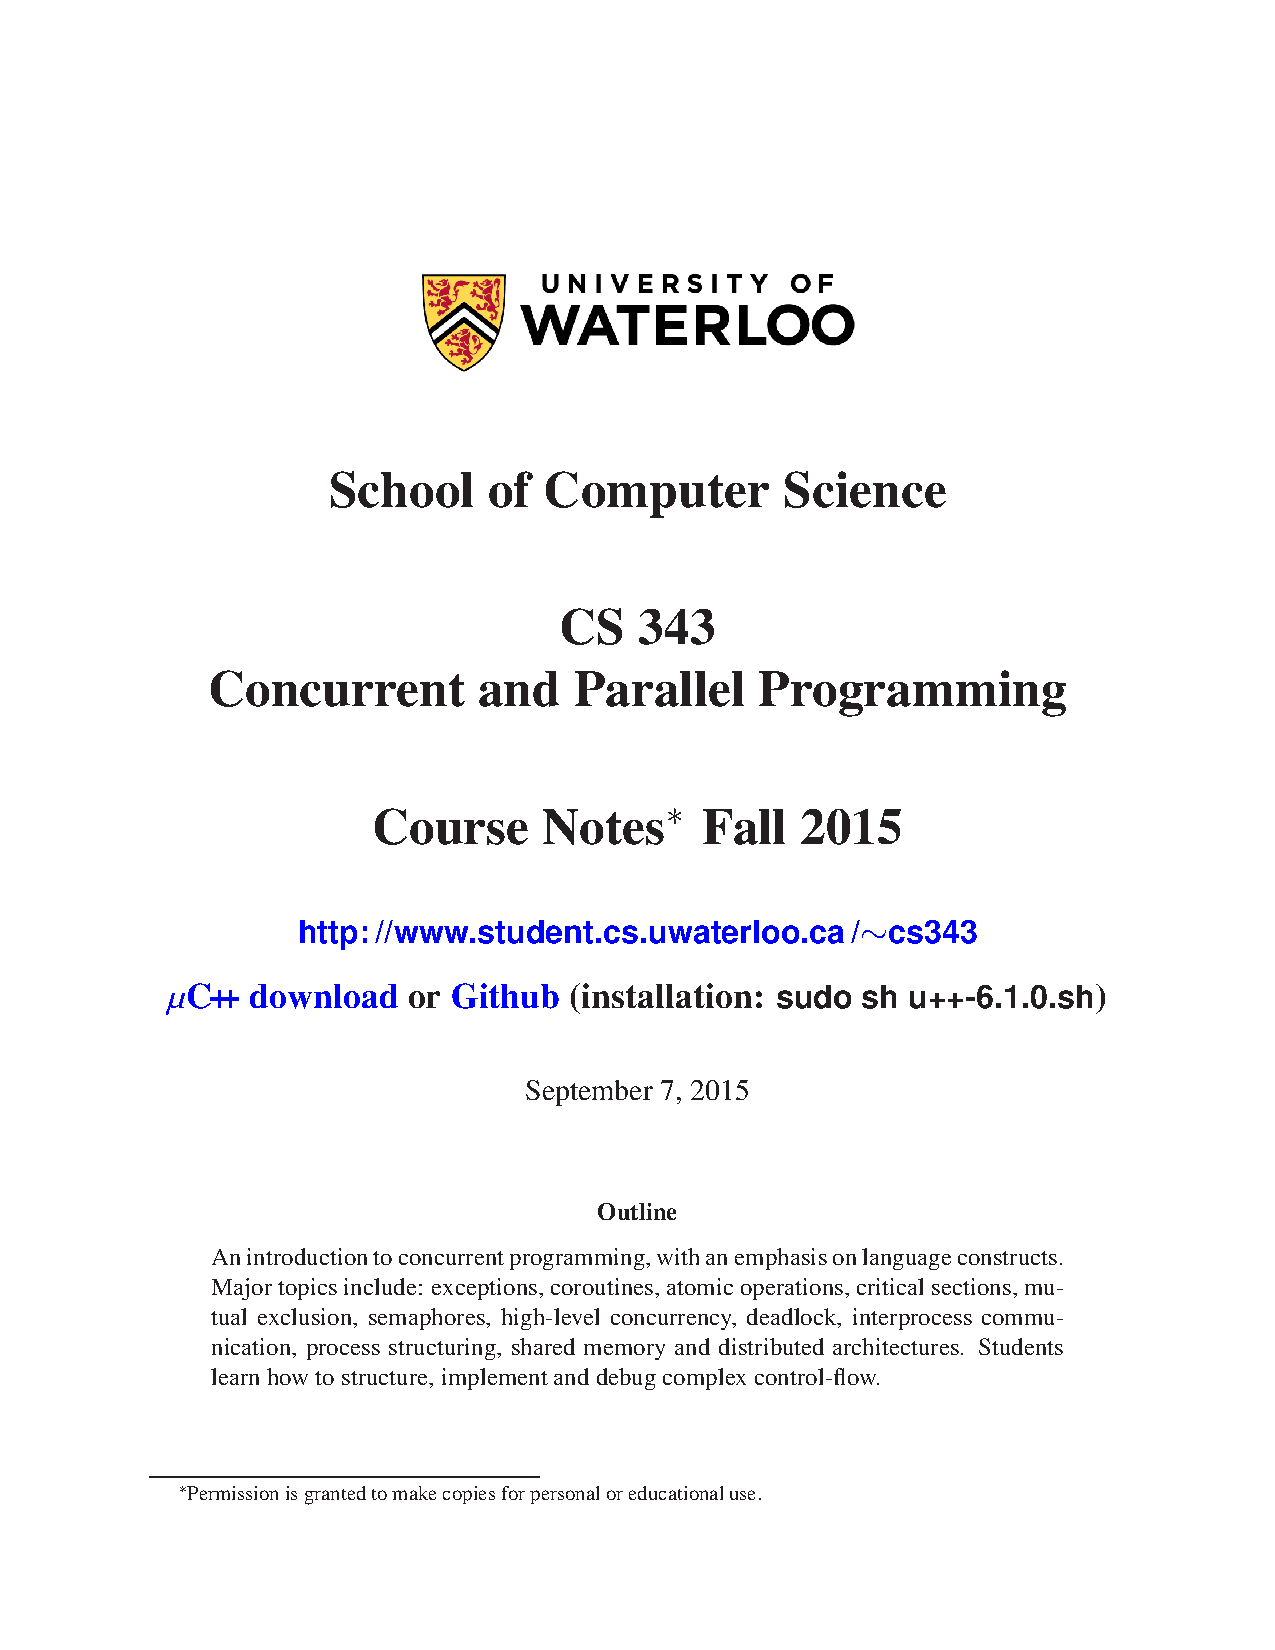
\includepdf[page=9-12]{../notes.pdf}
\textbf{Multiexit loop}
This is used when you need to break out in the middle of a loop.

\begin{itemize}
    \item get rid of duplicated code used for priming the loop (do the thing that might break before and at the end of the loop)
    \item get rid of conditional breaks in the else (there's no reason for it).
    \item get rid of flag variables, just break out of the middle of the loop.
\end{itemize}


\textbf{Static multiexit}
Exit multiple control structures. Micro c++ allow for labeled breaks. This way we can say break out of this specifically. In regular c++ we need to use gotos to do this. We like having the labels up top since its easier to find the loop that you are breaking out of. We want to label all exits so that we can be much more specific with our breaks.

Restrictions for goto:
\begin{itemize}
    \item not in a looping structure
    \item not goto into a control structure
    \item only for static multilevel exits
\end{itemize}

\subsection{Dynamic Memory Allocation}
Stack memory allocation should be the default. Unless:
\begin{itemize}
    \item if data must outlive its scope
    \item when the size of data is not known in advance (ex. vectors)
    \item when objects need to use their constructors
    \item when an object has a small stack (relative to the stack size of the routine)
    \begin{itemize}
        \item having big stacks waste a lot of virtual space(specifically for each thread)
    \end{itemize}
\end{itemize}

\textbf{make_unique} creates an autopointer for an object that cleans up all nested objects on falling out of scope (nested autopointers).


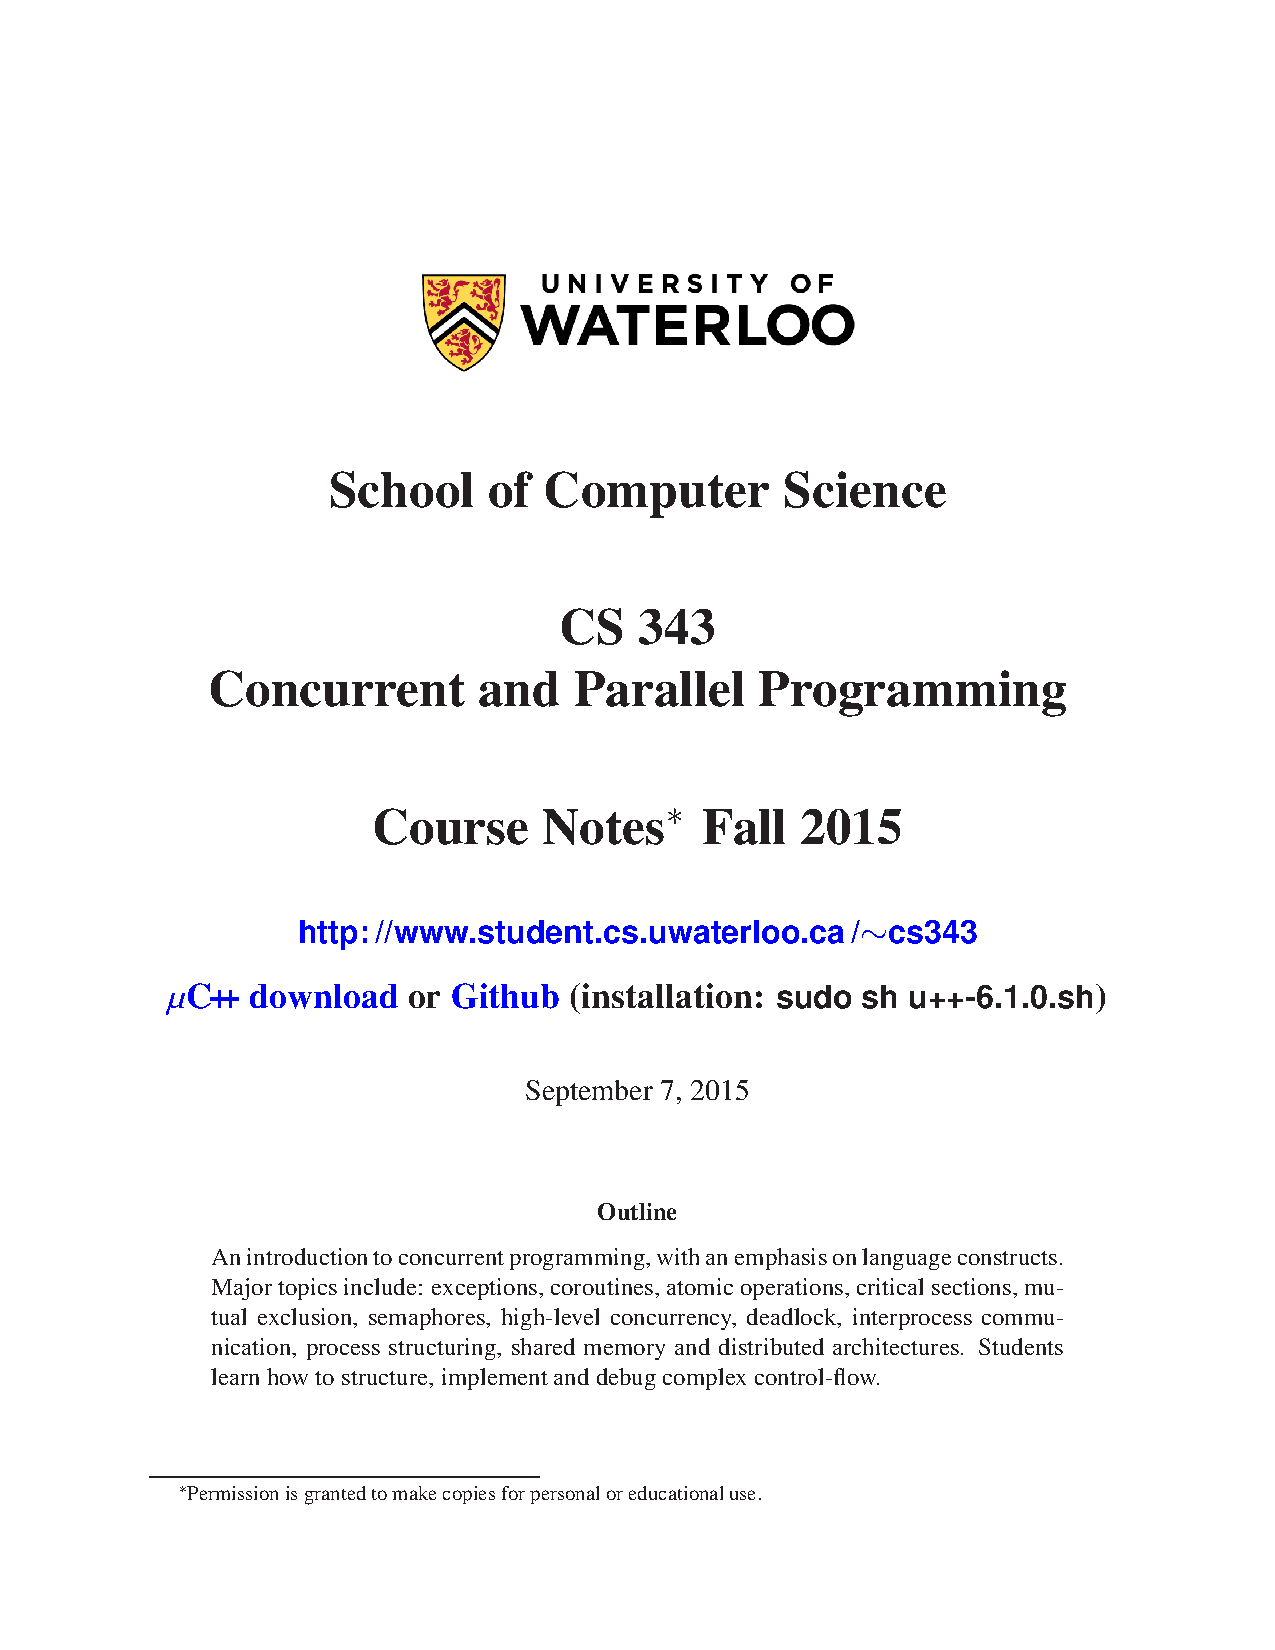
\includepdf[page=13-]{../notes.pdf}
\section{Exceptions}
\subsection{Dynamic multilevel exit}
We cannot have multilevel exits span routines, they must be in the same routine scope. Control flow must be determined by calls and returns. Similarly we cannot return to our parent's parent routine without resolving our parent.

We can have have an exceptional return. Passing * as parameters to a routine. These are named 1 and 2 and are alternative return points. When we return 1 or 2 we return to the line denoted by the parameter passed into the function call. These can be used to get around the above mentioned limitation when we cannot break to a location outside of our routine scope.

\subsection{Dynamic multilevel exit}
This uses call/return semantics to reverse the direction of normal routine calls.

Label L is a frame on the call stack and a place to return to.

When we call f(1) it will call goto L which will skip the call to S1. At L1 we can handle excpetional state before going to S1. Eventually we get to S1 and call g(1). We will eventually pop off a bunch of f and g stack frames until we get to h1 which will call goto L, at this point L=L2 so we go there and handle some shit before going to S2. L's value is associated with a specific invocation of h so some h's will be popped off the stack as well as f's and g's. Basically we are returning a specific dynamic location.

When we call goto L we keep searching through the stack until we find the frame that L is, if L is not on the stack we keep searching until we eventually terminate (end the stack).

If L is not set during a recursion of h we just skip right over it.

C has \textbf{jmp_buf} which is a jump variable, \textbf{setjmp} initializes it, and \textbf{longjmp} will jump there from anywhere. Basically these are how we implement the above code in c++. This can be used to develop our own exception handling functionality.

Nonlocal transfers are not very constrained which can fuck shit up.

\subsection{Traditional Approaches}
\textbf{Return Code} return a thing or a error value. This is the standard way of doing things. The problem with this is that its passive and programmers don't always check return values, we aren't forced to use it. Another problem is you cannot use this for any container structures (ex the at function of a vector could return anything so it has no return code since anything is valid). This also results in interleaving normal execution and exceptional execution since you need to check these codes and do shit if so.

\textbf{Status Flag} just set a global variable that anyone can see. This has the same problem as return codes since no one checks them.

\textbf{Fixup routine} this is a routine called when shit goes sideways in an attempt to fix it before returning. For instance when new fails it calls a fixup routine called newHandler which throws a bad alloc error when it fails. We could overwrite this and do some shenanigans. This can get clunky when lots of them are called (many different parameters) and nesting gets hairy

Frequently these are combined.






\end{document}
